% Reactive Language-Action Paper — CoRL/NeurIPS-style draft
% To use conference style, replace \documentclass{article} with the
% conference package (e.g. \usepackage{corl} or neurips_2024) and adjust
% the author/title macros accordingly.

\documentclass[11pt]{article}

\usepackage[margin=1in]{geometry}
\usepackage{graphicx}
\usepackage{amsmath,amssymb,amsfonts}
\usepackage{xcolor}
\usepackage{hyperref}
\usepackage[numbers,sort&compress]{natbib}
\usepackage{tikz}
\usetikzlibrary{arrows.meta,positioning,fit,backgrounds}

\hypersetup{colorlinks=true,linkcolor=blue,citecolor=blue,urlcolor=blue}

\title{GenToolReal: Generative Trajectory Prediction for\\Reactive Tool Manipulation via\\Language-Conditioned Flow Matching}

\author{
  Olivia Taylor\\
  Department of Computer Science\\
  Stanford University, United States\\
  \texttt{otaylor@stanford.edu}
  \and
  Tyler Lum$^{*}$\\
  Department of Computer Science\\
  Stanford University, United States\\
  \texttt{tylerlum@stanford.edu}
  \and
  Jeannette Bohg$^{*}$\\
  Department of Computer Science\\
  Stanford University, United States\\
  \texttt{bohg@stanford.edu}
}
\date{}

\begin{document}
\maketitle
{\let\thefootnote\relax\footnote{$^{*}$Advising role.}}

\begin{abstract}
We present a reactive tool-surface-conditioned Language-Action model for dexterous tool manipulation that predicts short-horizon tool trajectories from a natural-language instruction and the current state of the tool and the object it acts on.
We demonstrate the approach on brush sweeping and nail hammering, two behaviors whose useful tool surfaces---brush bristles and a hammer face---differ substantially.
We train it on procedurally generated demonstrations in which the planner repeatedly observes the scene, predicts the next stretch of motion, and lets the object move before observing again, so the policy learns to react as the scene changes.
We then refine the pretrained policy in simulation with group relative policy optimization (GRPO).
Trajectories are expressed in a contact frame anchored to the tool's functional surface, so the policy is not keyed to a hard-coded tool identity but grounded by the functional surface that should contact the world.
The predicted poses are handed to the SimToolReal controller, which executes them on a 22-DoF Sharpa five-fingered hand mounted on a 7-DoF KUKA iiwa 14 arm.
\end{abstract}

%==============================================================================
\section{Introduction}
%==============================================================================

Tool manipulation requires reasoning about functional contact geometry---where a tool meets the world, how it should be oriented, and how both evolve as the object being acted on moves.
End-to-end vision-language-action models~\cite{pi0,openvla,groot} learn visuomotor policies from large demonstration corpora but require substantial task-specific data and can be difficult to adapt to new tool--object interactions.
Modular approaches decouple semantic planning from low-level control~\cite{saycan,scaffolding,simtoolreal}, but prior language-conditioned \emph{goal} prediction predicts a single static configuration rather than motion that must be revised as the scene evolves.

We address \emph{reactive} tool manipulation: the system observes the current tool pose and object state, predicts a short-horizon trajectory, executes the beginning of it, and then reobserves and replans.
This pattern matches how people use tools---sweeping crumbs that scatter or hammering a nail that sinks incrementally.
The high-level trajectory is executed by the SimToolReal controller~\cite{simtoolreal} on a 22-DoF Sharpa five-fingered left hand mounted on a 7-DoF KUKA iiwa 14 arm, so the policy need only specify where and how the tool's working surface should move.

Our contributions are:
\begin{enumerate}
  \item A \textbf{contact-frame trajectory representation}---a sequence of waypoints, each giving a contact point, a contact normal, and an in-plane direction---anchored to the tool's functional surface. Because the policy reasons about where this working surface should contact the world rather than about a hard-coded tool identity, the same policy form can cover tools with different functional surfaces.
  \item \textbf{Procedural reactive demonstrations} for brush sweeping and nail hammering, in which an analytic expert is repeatedly re-queried from the updated scene state.
  \item A \textbf{single tool-surface-conditioned Language-Action model} trained with flow matching on reactive contact-frame trajectories and refined in simulation with GRPO.
  \item A \textbf{closed-loop deployment} in which the model replans from live observations and works with SimToolReal to execute brush sweeping and hammer nailing on a real robot.
\end{enumerate}

%==============================================================================
\section{Related Work}
%==============================================================================

\paragraph{Vision-Language-Action Models.}
Recent VLAs adapt large pretrained vision-language backbones for robot control by adding action prediction heads~\cite{pi0,pi05,pi07,openvla,groot,rt2}.
$\pi_0$~\cite{pi0} introduced a flow-matching action expert on a frozen VLM; OpenVLA~\cite{openvla} demonstrated competitive open-source fine-tuning on robot datasets; GR00T N1~\cite{groot} combines VLM reasoning with a diffusion action module.
Unlike these end-to-end image-conditioned policies, our model conditions on a compact symbolic state---the tool contact pose, the object pose, the destination, and the table---together with a language instruction, enabling lightweight deployment without a vision backbone at inference.

\paragraph{Language-Conditioned Manipulation.}
SayCan~\cite{saycan} grounds language plans in affordance functions; scaffolding approaches~\cite{scaffolding} use VLMs to decompose dexterous tasks into waypoints.
An earlier version of our system predicted a single goal configuration per step; here we instead predict full reactive trajectories that are re-queried from live state.

\paragraph{Flow Matching for Robot Control.}
Flow matching~\cite{flowmatching} learns vector fields that transport noise to data along straight-line paths, enabling stable training and fast sampling compared to diffusion-based action models~\cite{diffusionpolicy}.
$\pi_0$~\cite{pi0} applies flow matching to continuous action chunks; we apply it to short tool trajectories represented in a contact frame.

\paragraph{RL Fine-Tuning of Generative Policies.}
Group relative policy optimization~\cite{deepseekmath} normalizes rewards within sampled groups and updates the policy with a clipped surrogate, avoiding a learned critic.
We adapt it to a stochastic flow-matching policy by scoring sampled trajectories in closed-loop simulation.

\paragraph{Tool Manipulation and Simulation.}
SimToolReal~\cite{simtoolreal} provides an object-centric controller for zero-shot dexterous tool use; our model supplies the high-level trajectory that it tracks on the hand.
Procedural and simulation data generation~\cite{isaaclab,droid} complements real demonstrations; we generate expert reactive demonstrations analytically and use simulation for reinforcement learning and evaluation.

\paragraph{Keypoint and Contact Representations.}
CLIP~\cite{clip} grounds text labels in a shared embedding space; we use frozen CLIP encodings for instruction and object labels.
Each waypoint defines a right-handed contact triad from the contact normal and in-plane direction, which maps to a tool pose via a fixed tool-specific transform.

%==============================================================================
\section{Problem Formulation}
%==============================================================================

At each replan, the system receives a natural-language instruction $\ell$, the current tool contact pose (a contact point $\mathbf{p}_c$, contact normal $\mathbf{n}$, and in-plane direction $\mathbf{s}$ orthogonal to $\mathbf{n}$), the object pose, the destination, and a table reference.
The policy predicts a trajectory of $K{=}15$ contact-frame waypoints:
\begin{equation}
  \hat{\mathbf{Y}} = [\hat{\mathbf{y}}_1, \ldots, \hat{\mathbf{y}}_K], \quad
  \hat{\mathbf{y}}_i = [\hat{\mathbf{p}}_{c,i};\ \hat{\mathbf{n}}_i;\ \hat{\mathbf{s}}_i] \in \mathbb{R}^9.
\end{equation}
Each waypoint defines a contact-frame rotation $\mathbf{R}_i = [\hat{\mathbf{s}}_i,\ \hat{\mathbf{n}}_i \times \hat{\mathbf{s}}_i,\ \hat{\mathbf{n}}_i]$ and, with a fixed transform from the contact frame to the tool root, yields a 6-DOF tool goal pose for the controller.

\paragraph{Closed-loop execution.}
A single controller executes the beginning of the predicted trajectory---either a fixed number of leading waypoints or as many as fit in a fixed time window---then reobserves the tool and object state and queries the model again.
Training data mirrors this loop: each scene is a sequence of replanning steps, each pairing the current state with the expert's next short-horizon plan.

%==============================================================================
\section{Method}
%==============================================================================

\subsection{Contact-Frame Trajectory Representation}
\label{sec:contact_frame}

We represent the tool at each waypoint by the contact point on its functional surface, the outward contact normal, and an in-plane direction $\mathbf{s}$ describing the orientation of that surface (for example, the direction the brush sweeps or the orientation of the hammer face).
Normals and in-plane directions are unit vectors; at post-processing, $\mathbf{s}$ is projected orthogonal to $\mathbf{n}$ and renormalized.
Anchoring the trajectory to the working surface---rather than to a particular tool identity---lets the same representation describe tools with different functional surfaces, since the policy reasons about how that surface should contact the world.
The representation is compact (nine numbers per waypoint), differentiable for flow matching, and composes directly with SimToolReal's object-centric tracking.

\subsection{Model Architecture}
\label{sec:architecture}

The policy is a self-attention transformer with hidden size $512$, four layers, and eight heads.
Its input is a short sequence of tokens:
\begin{center}
\texttt{[instruction, tool, object, destination, table, noisy trajectory]},
\end{center}
where object/destination tokens are omitted when not relevant to a task.
Each semantic label is encoded by a frozen CLIP ViT-B/32 text encoder~\cite{clip} and projected to the model dimension; each position passes through a small MLP on normalized coordinates and is added to its label embedding.
The final token carries the current noisy trajectory.
Each transformer block applies pre-norm self-attention followed by an MLP, with an adaptive normalization conditioned on the flow-matching timestep.
The hidden state of the trajectory token is projected to the predicted flow velocity.

\subsection{Flow-Matching Objective and Inference}
\label{sec:flow}

Training uses conditional flow matching~\cite{flowmatching}.
For an example with normalized target trajectory $\mathbf{x}_1$,
\begin{align}
  \mathbf{x}_0 &\sim \mathcal{N}(\mathbf{0}, \mathbf{I}), \quad t \sim \mathcal{U}(0,1), \\
  \mathbf{x}_t &= (1-t)\mathbf{x}_0 + t\mathbf{x}_1, \quad \mathbf{v}^* = \mathbf{x}_1 - \mathbf{x}_0,
\end{align}
and the model minimizes $\|\hat{\mathbf{v}}_\theta(\mathbf{x}_t, t, \text{cond}) - \mathbf{v}^*\|^2$.
Only contact positions are affine-normalized; normals and in-plane directions are trained as raw 3-vectors and normalized after integration.
At inference we integrate the learned ODE with $30$ Euler steps, draw four independent samples, and average their final trajectories.

\subsection{Procedural Reactive Demonstrations}
\label{sec:data}

We generate demonstrations for the two demonstrated tasks with analytic expert planners:
\begin{itemize}
  \item \textbf{Sweep with brush}: push loose debris across the table into a receptacle.
  \item \textbf{Hammer nail}: strike a nail head until it reaches a target depth.
\end{itemize}
The representation is intended to support additional functional surfaces, but this paper reports reliable results only for the brush and hammer settings.

\paragraph{Reactive demonstrations.}
Each scene is rolled out as a closed loop.
At every step the expert plans a 15-waypoint trajectory, executes the first few waypoints, and lets the scene update before planning again.
Between steps we perturb the scene---jitter or knock the object, scatter debris, or land a weak hammer hit---so the expert must recover, and the resulting demonstrations teach the policy to react rather than to follow a fixed script.
Each step yields one training example that pairs the current observation with the expert's next plan.

\paragraph{Natural-language instructions.}
Each scene is specified by a free-form natural-language instruction sampled once and reused across that scene's replanning steps.
To encourage generalization across phrasing rather than memorizing a fixed command, we generate a large and diverse instruction set per task by combining many templated sentence structures with varied synonyms for the tool, the object, and the destination (for example, ``sweep the crumbs into the dustpan'' versus ``brush the debris toward the tray'').
This exposes the model to a wide range of wordings for the same underlying task.

\paragraph{Scale.}
The demonstrated tasks are balanced at the example level: per-task data caps are chosen so that brush sweep and hammer nailing contribute comparable numbers of training examples.
Labels are produced analytically; simulation is used only for reinforcement learning and evaluation.

\subsection{Joint Pretraining}
\label{sec:pretrain}

We pretrain on the reactive demonstrations, concatenating brush and hammer trajectories and shuffling across tasks, with a global per-axis normalization of contact positions computed over the combined data.
Training runs for ten epochs with batch size $128$ and AdamW (learning rate $5{\times}10^{-4}$, brief warmup then cosine decay).
This checkpoint is the starting point for reinforcement learning.

\subsection{GRPO Simulation Fine-Tuning}
\label{sec:grpo}

We refine the policy with group relative policy optimization~\cite{deepseekmath,ppo}.
For each scene the policy samples several trajectories by integrating the flow with injected noise and recording the probability of the sampled path.
Each trajectory is executed in closed-loop simulation and assigned a scalar task reward.
Advantages are normalized within each scene's group of samples,
\begin{equation}
  A_i = \frac{r_i - \bar{r}}{\sigma_r + \epsilon},
\end{equation}
and the policy is updated with a clipped likelihood-ratio surrogate plus a penalty that keeps it close to the pretrained model.
A single training run samples brush and hammer scenes during refinement, and checkpoints are saved periodically.

\paragraph{Per-task rewards.}
\begin{itemize}
  \item \textbf{Brush}: reward for the swept object reaching the goal region, combined with a term for how well the hand tracked the requested trajectory.
  \item \textbf{Hammer}: reward for how far the nail is driven toward its target depth, with full credit on reaching it.
\end{itemize}

%==============================================================================
\section{Closed-Loop Deployment}
\label{sec:deploy}
%==============================================================================

At deployment a single closed-loop controller handles brush sweeping and nail hammering.
It observes the current tool and object pose, predicts a 15-waypoint trajectory, and converts each contact-frame waypoint into a tool goal pose, which it hands to SimToolReal for execution on the hand.
Tool and object poses are estimated with FoundationPose~\cite{foundationpose}---the same pose estimator SimToolReal uses for tool tracking---so perception integrates cleanly across the two systems with no additional calibration.
It then executes the beginning of the plan---either a fixed number of waypoints or as many as fit in a short time window---reobserves, and replans, repeating until the object reaches its destination.
The model operates in its own world frame, so observations are transformed in from the robot frame and predicted poses are transformed back out before execution.
The same package drives both the real robot and an interactive visualization used for development, in which the predicted trajectory and tool poses can be inspected before running on hardware.

%==============================================================================
\section{Experiments}
\label{sec:experiments}
%==============================================================================

\paragraph{Evaluation setup.}
Simulation evaluation uses the same closed-loop protocol as reinforcement learning, with task success defined as in Section~\ref{sec:grpo} (debris in the goal region or nail driven to depth).
On the real robot, the closed-loop controller drives SimToolReal and success is measured by task completion.

\paragraph{Qualitative results.}
The pretrained model produces coherent brush-sweep arcs and hammer strikes that descend toward the nail.
On the real robot, closed-loop replanning yields continuous tool motion across replans for multiple brush instances/appearances and for hammer nailing.
These rollouts support a tool-instance-independent framing for demonstrated brush variants, while the broader claim is that the policy is grounded by the functional surface/contact frame rather than by a hard-coded tool identity.

\begin{figure}[t]
  \centering
  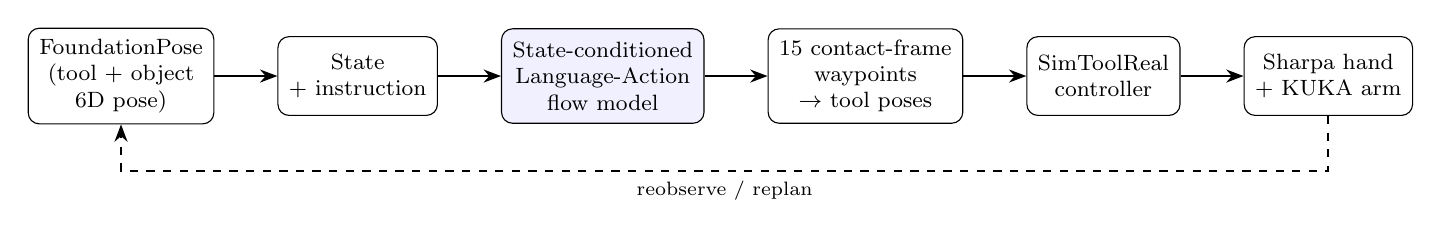
\begin{tikzpicture}[
      node distance=6mm and 8mm,
      box/.style={draw, rounded corners, align=center, inner sep=4pt, minimum height=10mm, font=\footnotesize},
      model/.style={box, fill=blue!6, minimum height=12mm},
      arr/.style={-{Stealth[length=2.2mm]}, thick},
    ]
    \node[box] (perc) {FoundationPose\\(tool + object\\6D pose)};
    \node[box, right=of perc] (state) {State\\+ instruction};
    \node[model, right=of state] (vla) {State-conditioned\\Language-Action\\flow model};
    \node[box, right=of vla] (wp) {15 contact-frame\\waypoints\\$\to$ tool poses};
    \node[box, right=of wp] (sim) {SimToolReal\\controller};
    \node[box, right=of sim] (robot) {Sharpa hand\\+ KUKA arm};
    \draw[arr] (perc) -- (state);
    \draw[arr] (state) -- (vla);
    \draw[arr] (vla) -- (wp);
    \draw[arr] (wp) -- (sim);
    \draw[arr] (sim) -- (robot);
    % replan feedback loop
    \draw[arr, dashed] (robot.south) -- ++(0,-7mm) -| node[pos=0.25, below, font=\scriptsize] {reobserve / replan} (perc.south);
  \end{tikzpicture}
  \caption{System overview. FoundationPose estimates tool and object poses; together with the instruction these form the symbolic state for the state-conditioned Language-Action model, which predicts a contact-frame trajectory. Waypoints are converted to tool goal poses and tracked by SimToolReal on the Sharpa hand and KUKA arm. The loop closes by reobserving and replanning.}
  \label{fig:system}
\end{figure}

\begin{figure}[t]
  \centering
  
\includegraphics[width=0.46\linewidth]{figures/hammer_control_frame.png}\hfill
  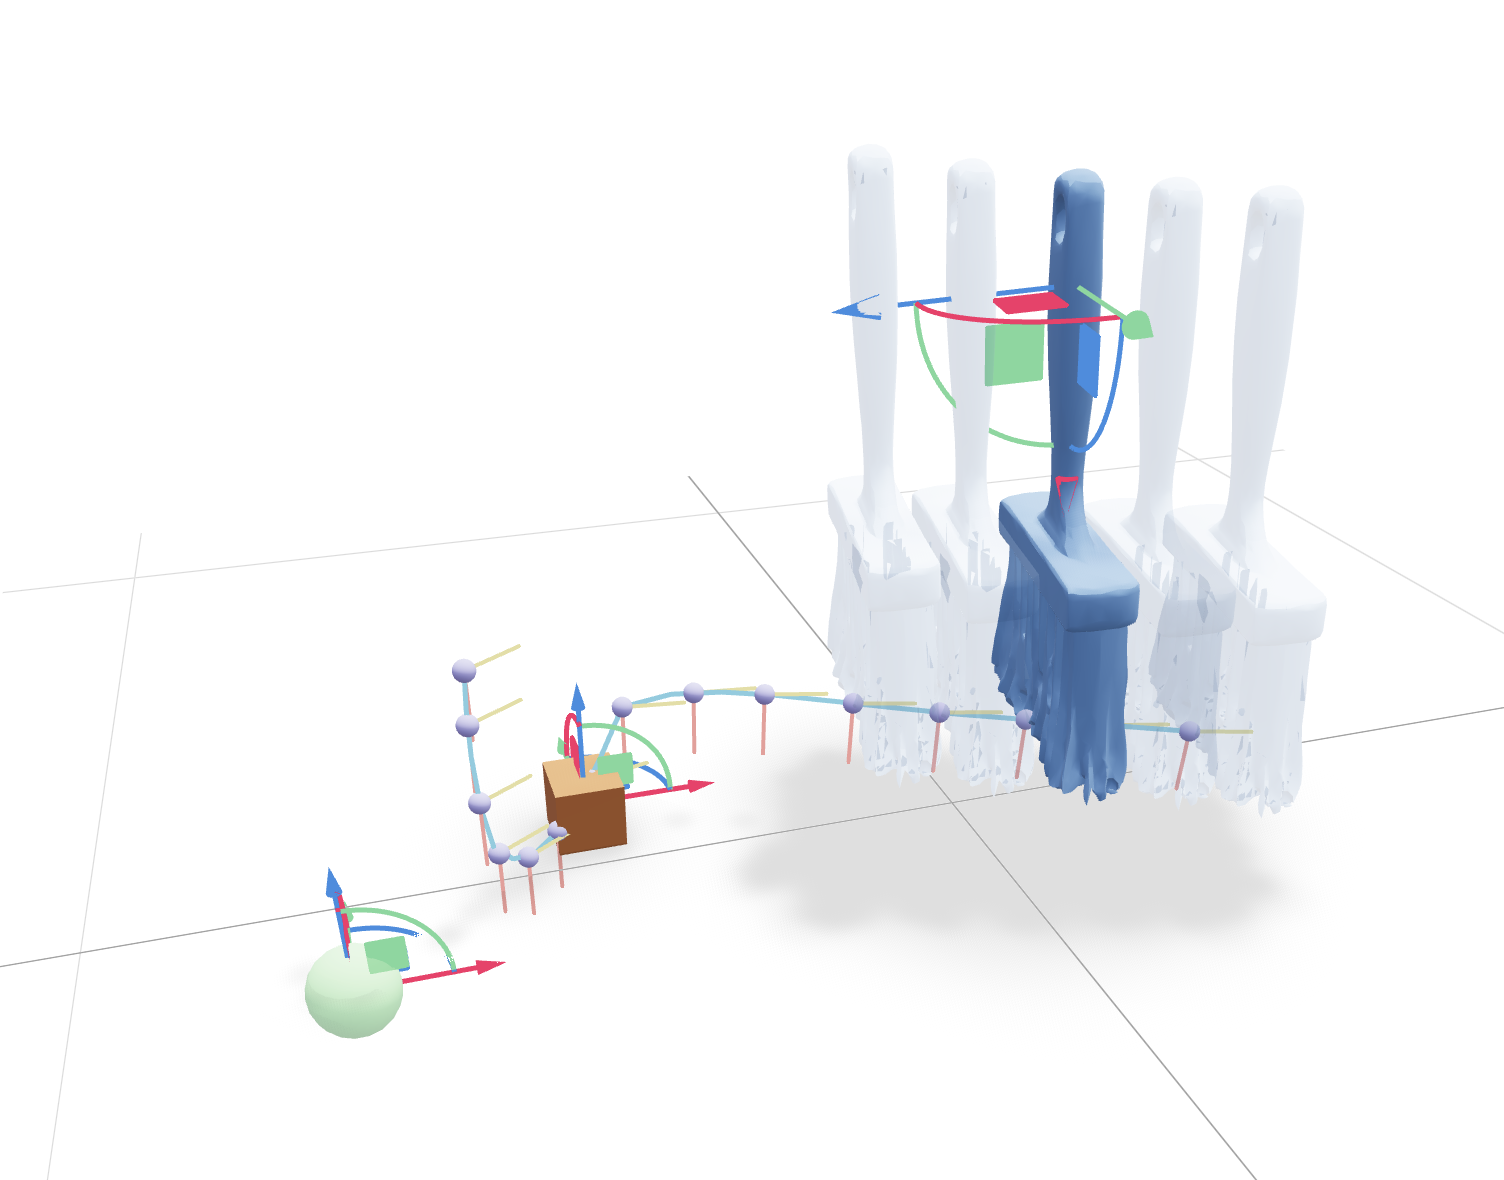
\includegraphics[width=0.46\linewidth]{figures/brush_trajectory.png}
  \caption{Left: the contact-frame definition for the hammer---a contact point with its normal and in-plane direction anchored to the tool's functional surface. Right: a predicted brush-sweep trajectory of contact-frame waypoints.}
  \label{fig:tasks}
\end{figure}

%==============================================================================
\section{Limitations and Future Work}
%==============================================================================

\paragraph{Model.}
The model does not condition on images, so visual obstacles and fine geometry must be inferred from sparse state.
Training labels come from analytic experts rather than human or simulated rollouts, which may not cover every failure mode, and the reinforcement-learning rewards are task-specific and bounded by simulation.
Robot time was limited, so our real-robot rollouts cover blue-brush and red-brush sweep variants and claw-hammer nailing.
Exploratory spatula-flip and spoon-pour extensions require more robust training, domain randomization, and reward design before they should be presented as demonstrated results.

\paragraph{Perception and execution failures.}
Because both our system and SimToolReal rely on FoundationPose for pose estimation, tracking errors propagate end-to-end: the SimToolReal policy would occasionally lose the object during execution, after which the predicted goals no longer matched reality.

\paragraph{Orientation behavior.}
On some replans the policy predicts an orientation rotated by roughly $180^\circ$ about the contact normal---it negates the in-plane direction even though the contact point and normal are unchanged---producing a discontinuous jump in the tool's goal orientation.
When not fully corrected, this jump made the arm try to move too fast to catch up and sometimes drop the object.
We mitigate it at deployment by aligning each new plan's orientation to the previous one and choosing the in-plane direction closest to it, without otherwise changing the contact frame, but this is a workaround for behavior the policy should not exhibit in the first place.
Relatedly, the policy tended to prefer a particular tool orientation and would force the trajectory to follow it even when another orientation would have worked equally well (for example, sweeping the brush from the opposite direction).

\paragraph{Future work.}
We expect the orientation preferences and discontinuities to respond to more aggressive domain randomization during training and to a penalty for extra steps in simulation (discouraging the policy from committing to a single orientation and from taking redundant motions), alongside removing the discontinuities at their source through orientation-aware training, image conditioning, and larger-scale reinforcement learning.
Future work should also revisit spatula flipping and spoon pouring as contact-frame extensions once the training distribution, simulation rewards, and domain randomization are strong enough to support reliable rollouts.

%==============================================================================
\section{Conclusion}
%==============================================================================

We presented a reactive tool-surface-conditioned Language-Action model for dexterous tool manipulation that predicts contact-frame tool trajectories from language and the current scene state, trained on procedural reactive demonstrations for brush sweeping and nail hammering, refined with GRPO in simulation, and deployed in a closed loop that works with SimToolReal to execute on a dexterous hand.
The system moves from single-goal prediction to continuous closed-loop trajectory generation, with a functional-surface-conditioned representation that bridges learning and low-level execution without keying the policy to a hard-coded tool identity.

%==============================================================================
\section*{Acknowledgments}
%==============================================================================

We thank the SimToolReal team for the low-level execution stack and simulation environments.

\bibliographystyle{plainnat}
\bibliography{references}

\end{document}
